\chapter{Results}
\label{sec:results}

In this Chapter, results of GAT-Denoiser are presented.
First, some small experiments are presented, which do not work on full dataset.
These experiments have been done to find the best suitable architecture and to 
familiarize with the problem and its structure.
Second, a few large experiments are presented, which work on full dataset.
During small and large experiments, some interesting findings are illustrated and GAT-Denoiser
is compared to U-Net and block-matching and 3D filtering (BM3D)~\cite{bm3d}.


\section{Dataset}
GAT-Denoiser is tested on LodoPaB-CT~\cite{lodopab-dataset} dataset, which is a 
benchmark dataset for low-dose ct reconstruction methods and therefore well suited for our domain.

The dataset consists of 35820 train images and 3553 test images.
All these images are having resolution 64.

\begin{figure}[H]
  \centering
  \hfill
  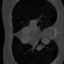
\includegraphics[width=0.2\textwidth]{ct_im_0.png}
  \hfill
  
\includegraphics[width=0.2\textwidth]{ct_im_1.png}
  \hfill
  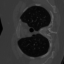
\includegraphics[width=0.2\textwidth]{ct_im_2.png}
  \hfill
  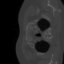
\includegraphics[width=0.2\textwidth]{ct_im_3.png}
  \hfill
  \caption{Some train images of LodoPaB-CT dataset.}
\end{figure}



\section{Project setup}
Python source code of the project is available on GitHub\footnote{https://github.com/cedricmendelin/master-thesis}.
Several python packages are used in the code, Pytorch geometric\footnote{https://pytorch-geometric.readthedocs.io/en/latest/} 
for neural network configuration, Operator Discretization Library\footnote{https://odlgroup.github.io/odl/} for Radon transform and FBP, 
and last, Weight \& Bias\footnote{https://wandb.ai/site} to gather results in a convenient way.

Training of GAT-Denoiser has been performed on the HPC-cluster scicore of the University of Basel.
During training, up to 4 titanx GPUs with 12 GB RAM have been used.


\paragraph{Radon transform:}
Radon transform will be applied in GAT-Denoiser and sampling points have been fixed to 64, so $s \in \mathbb{R}^64$.
Further, projection angles $\theta$ are sampled within interval $[0, \pi]$.
The number of observation is the size of our input graph, where typically 1024 nodes are used, but 
there are some experiments with other figures.


\paragraph{GAT settings:}
During experiments, in GAT-layers ELU was used as activation function.
Further, dropout is used as regularization term and fixed to XX.
During training, adam optimizer was with fixed learning rate $0.01$ and weight decay $0.0005$.


\paragraph{Performance metrics}:
During evaluation, two main metrics are considered.
First, \textit{Loss} is used, which refers to the average $\ell$-2 distance between original object and reconstruction.
Second, \textit{SNR} is used, which refers to SNR in dB of reconstruction, compared to original object.
Further, visual results are presented and can be seen as a third metric.

To make notation clear, \textit{SNR} in this Chapter refers to SNR computed from denoised reconstruction and original object 
and always shows an average on a test set for a specific algorithm or model.
Contrary, $\textit{SNR}_y$ is used to express the level of noise during training or validation, 
where SNR is computed from clean and noisy observation.

\paragraph{U-Net training:}
As described in Section~\ref{sec:unet} \textit{\nameref{sec:unet}}, U-Net will be part of our model.
Therefore, U-Net was pre-trained on the LodoPaB-CT training dataset, with 128 channels in the first contracting step. 
In total, 4 steps have been computed, which results in 1024 channels as output of last contracting step.
During training, noise was sampled from normal distribution to reach SNR in the interval $[0, -10]$ and was added to the observation (sinogram). 
In total, model was trained for 200 epochs.

\paragraph{BM3D:}
BM3D is a powerful and lightweight algorithm for image denoising. 
It is not neural network based and was the defacto state-of-the-art before neural network outperformed
BM3D. Therefore, it is an interesting baseline to compare with.

In the GAT-Denoiser pipeline, first, observations will be denoised ,and second, reconstruction is computed.
Therefore, BM3D can be applied at two different steps. First, it can be used to denoise sinogram
and forward denoised sinogram to FBP, which is how GAT-Denoiser work. Secondly, FBP can be
computed with noisy sinogram and output can be forwarded to BM3D, which will denoise reconstruction.
In the following term \textit{BM3D sinogram} and \textit{BM3d reconstruction} 
are used to distinguish between the two approaches.

\section{Small Experiments}
For small experiments, not the complete LodoPaB-CT dataset was considered, but only 1024 train images
and 100 validation images. 
Further, evaluated GAT-Denoiser models presented in this Section have been trained for 200 epochs.

\subsection{Baseline}

In Table~\ref{tab:baseline-small}, baseline results for FBP, BM3D sinogram, BM3D reconstruction and U-Net can be found.
Noise was added to reach $\textit{SNR}_y$ of 0, -5, -10 and -15 dB.

As expected, reconstruction FBP performs the worst, as it only reconstructs from noisy observation. 
For higher SNR 0 dB BM3D outperforms U-Net, which lays down the power of BM3D.
But, for lower SNR's -5 to -15 U-Net performs better and is the baseline to beat.

\begin{table}[H]
  \centering
  \begin{threeparttable}
    \begin{tabular}{l|cc|cc|cc|cc}
    \toprule
    \textbf{Algorithm} & \multicolumn{2}{c|}{\snrh{ 0}} & \multicolumn{2}{c|}{\snrh{ -5}} & \multicolumn{2}{c|}{\snrh{ -10}} & \multicolumn{2}{l}{\snrh{ -15}} \\
                       & \textbf{Loss} & \textbf{SNR}  & \textbf{Loss} & \textbf{SNR}  & \textbf{Loss} & \textbf{SNR} & \textbf{Loss} & \textbf{SNR} \\ 
    \midrule
    FBP                 &  1041.6          &  4.81            & 1772.8         & 0.0           & 3105.6          & -4.96          & 5495.2       & -9.94       \\ \hline
    BM3D sinogram       &  662.2           &  9.30            & 909.5          & 6.13          & 1285.2          & 2.93           & 1884.9       & -0.50       \\ \hline
    BM3D reconstruction &  \textbf{604.2}  &  \textbf{10.15}  & 840.4          & 6.81          & 1283.1          & 2.89           & 2079.1       & -1.42       \\ \hline
    U-Net               &  674.9           &  9.03            & \textbf{711.5} & \textbf{8.17} & \textbf{711.5}  & \textbf{8.17}  & \textbf{1224.9}       & \textbf{3.10}        \\ 
    \midrule
    \end{tabular}

  \end{threeparttable}

  \caption{Baseline results small experiments: the best result in column is marked bold. }
  \label{tab:baseline-small}
\end{table}

Further, for \snry 0 dB, reconstruction of a single test image for all baseline algorithms is illustrated in Figure~\ref{fig:baseline_small}.

  \begin{figure}[H]
    \label{fig:baseline_small}
    % \centering
    \hfill
    \subbottom[\label{fig:test_clean}]{
\includegraphics[width=0.15\textwidth]{baseline_small_clean.png}}
    \hfill
    \subbottom[\label{fig:test_fbp}]{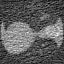
\includegraphics[width=0.15\textwidth]{baseline_small_fbp.png}}
    \hfill
    \subbottom[\label{fig:test_bm3d_sino}]{
\includegraphics[width=0.15\textwidth]{baseline_small_bm3d_sino.png}}
    \hfill
    \subbottom[\label{fig:test_bm3d_reco}]{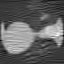
\includegraphics[width=0.15\textwidth]{baseline_small_bm3d_reco.png}}
    \hfill
    \subbottom[\label{fig:test_unet}]{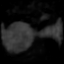
\includegraphics[width=0.15\textwidth]{baseline_small_unet.png}}
    \hfill
	\caption{Example test image baseline reconstructions for \snry 0 dB:\\
  \ref{fig:test_clean} clean test image, \ref{fig:test_fbp} FBP reconstruction, \ref{fig:test_bm3d_sino} BM3D sinogram, 
  \ref{fig:test_bm3d_reco} BM3D reconstruction, \ref{fig:test_unet} U-Net reconstruction}
\end{figure}

  \subsection{Input graph structure}
  In the following Section, experiments with different input graphs are presented.
  As the domain of interest is the input graph and its size, and therefore the number of observations, 
  some other parameters are fixed for all experiments.
  First, U-Net was deactivated, resulting reconstruction is defined as FBP solely.
  Further, GAT-Denoiser has been set to 3 layers with GAT single head and convolution 
  with one channel, kernel size 3 and padding 1. 
  If nothing else noted, noise was added to reach \snry 0 dB.

  The input graph structure is important for GAT learning. As described in Section~\ref{sec:manifold_ct_cryoEM}
  \textit{\nameref{sec:manifold_ct_cryoEM}} the computed tomography underlying manifold is assumed to be a circle 
  in the clean case, therefore our graph is fixed as a circle graph. 
  Moreover, learning is expected to fail when learning on a random graph.

  Further, the neighborhood size for k-NN graphs is explored, as it is expected to be not easy to find 
  good values for parameter $k$.

  \paragraph{Does learning fail with random graph?}
  Yes it does.

  During this experiment, two models with different input graphs, but same size 1024 nodes have been trained.
  First, a k-NN graph with $k=10$ was defined as input, therefore, around 1\%  of all nodes are connected to a single node.
  Second, a random Erdős–Rényi graph with $p=0.01$ has been evaluated, where every node is 
  approximately connected to 1\% of all available nodes. Consequently, both graphs have approximately the same amount of edges.
  
  In the experiment, random Erdős–Rényi graph fails to learn denoising and k-NN starts to capture some details.
  Table~\ref{tab:input_graph} shows Loss and SNR and in Figure~\ref{fig:input_graph_small} example reconstruction is illustrated.

  \begin{table}[H]
    \centering
      \begin{tabular}{l|cc}
      \toprule
      \textbf{Input graph} & \textbf{Loss} & \textbf{SNR}  \\ 
      \midrule
      Erdős–Rényi graph with $p=0.01$    &  1509.3          &  1.3   \\ \hline
      K-NN graph with $k=10$       &  718.74          &  7.7    \\ \hline
      \midrule
      \end{tabular}
    \caption{Loss and SNR for random graph vs. k-NN graph. }
    \label{tab:input_graph}
  \end{table}
  
  \begin{figure}[H]
    \label{fig:input_graph_small}
    % \centering
    \hfill
    \subbottom[\label{fig:small_experiment_clean2}]{
\includegraphics[width=0.2\textwidth]{baseline_small_clean.png}}
    \hfill
    \subbottom[\label{fig:small_experiment_random_graph}]{
\includegraphics[width=0.22\textwidth]{random__graph_small_experiment.png}}
    \hfill
    \subbottom[\label{fig:small_experiment_knn_graph}]{
\includegraphics[width=0.2\textwidth]{knn__graph_small_experiment.png}}
    \hfill
	\caption{Example test image reconstructions for different input graphs:\\
  Where \ref{fig:small_experiment_clean2} is clean object, 
  \ref{fig:small_experiment_random_graph} reconstruction with  Erdős–Rényi input graph with $p=0.01$ and 
  \ref{fig:small_experiment_knn_graph} reconstruction K-NN input graph with $k=10$.
  }
\end{figure}


  \paragraph{Does result improve with large graph size?}
  Slightly.
  For this question to answer, multiple models have been trained for graphs with size 512, 1024 and 2048 
  as well as different k-NN parameters $(2,6,8,10,20)$.

  In Table~\ref{tab:graph_knn} results are presented. 
  So yes, larger graph size improve our model. 
  But, training is also more expensive regarding execution time. 
  Therefore, for all upcoming experiments graph size is fixed to 1024, as it looks like a good
  value in between, with good reconstruction result but also not too much training time.
  
  \begin{table}[H]
    \centering
      \begin{tabular}{l|ccc}
      \toprule
      \textbf{Input graph size} & \textbf{Loss} & \textbf{SNR} & \textbf{Training time (s)}  \\ 
      \midrule
      512  &  732.7    &  7.6  & 2678 s \\ \hline
      1024 &  696.1    &  8.1  & 4216 s \\ \hline
      2048 &  628.8    &  8.9  & 7609 s  \\ \hline
      \midrule
      \end{tabular}
    \caption{Loss and SNR for different input graph sizes, which refer to the average of different k-NN parameters.}
    \label{tab:graph_knn}
  \end{table}

  \paragraph{What is a good parameter k for k-NN graph construction?}

  As described in Chapter~\ref{sec:manifold_ct_cryoEM} \textit{\nameref{sec:manifold_ct_cryoEM}},
  it is not easy to determine parameter $k$ in general.
  Therefore, multiple models have been trained with different $k=(2,6,8,10,20)$
  as well as different \snry range (0 dB and -10 dB)


  In Table~\ref{tab:small_knn_snr}, result of calculated models are illustrated.
  First, input graph resulting from $k=2$ performs surprisingly good for SNR 0 dB as well as -10 dB.


  \begin{table}[H]
    \centering
    \begin{tabular}{l|cc|cc}
      \toprule
      \textbf{K-NN parameter k} & \multicolumn{2}{l|}{\snrh{ 0}} & \multicolumn{2}{l|}{\snrh{ -10}}  \\
                         & \textbf{Loss} & \textbf{SNR} & \textbf{Loss} & \textbf{SNR} \\ 
      \midrule
      2    &  \textbf{609.2}  &  \textbf{9.15}  & 741.4  & 7.49   \\ \hline
      6    &  650.3           &   8.58          & 919.8  & 5.57   \\ \hline
      8    &  683.0           &   8.17          & 859.4  & 6.19   \\ \hline
      10   &  718.7           &   7.72          & 954.8  & 5.25   \\ \hline
      20   &  819.3           &   6.62          & 1028.4 & 4.63   \\  
      \midrule
    \end{tabular}
  
    \caption{Different k-NN values for \snry 0 dB and -10 dB }
    \label{tab:small_knn_snr}
  \end{table}

\textbf{TODO: Argue why from now on k-nn = 8}


\subsection{GAT parameters}
In this Section, experiments are executed with focus on GAT and it's parameters.
Mainly, two parameters are important: number of heads and number of GAT layers.

To recap, the k-hop neighborhood in a GNN is defined by the number of layers.
Therefore, number of layers is expected to keep rather low. The dataset has only resolution 64
and consequently, it is expected that too many layers will average a too large neighborhood.

Further, number of heads determines if the learned weight matrix is divides into several parts.
The larger the number of heads, the smaller are the parts of the weight matrix.
Overall, larger number of heads is expected to smoothen denoising, but too large values
will divide weight matrix in too many parts, leading to bad results.

During GAT experiments, graph size 1024 was used and parameter $k=8$.
Further, convolution was applied with a single channel, kernel size = 3 and padding 1.
As focus is on GAT parameters, U-Net was not used during these experiments.
Further, multiple experiments with layers = $(2,3,4,6)$ and heads = $(1,2,4,8,16)$ have been evaluated, 
where results can be found in Table~\ref{tab:small_gat_results}.

\begin{table}[H]
  \centering
  \begin{tabular}{l|cc|cc|cc|cc|cc}
    \toprule
    \textbf{Heads} & \multicolumn{2}{c|}{\footnotesize \textbf{2 Layers}} & \multicolumn{2}{c|}{\footnotesize \textbf{3 Layers}} & \multicolumn{2}{c|}{\footnotesize \textbf{4 Layers}} & \multicolumn{2}{c|}{\footnotesize \textbf{6 Layers}} & \multicolumn{2}{c}{\footnotesize \textbf{Average}} \\
                   & \textbf{Loss} & \textbf{SNR} & \textbf{Loss} & \textbf{SNR} & \textbf{Loss} & \textbf{SNR} & \textbf{Loss} & \textbf{SNR} & \textbf{Loss} & \textbf{SNR} \\ 
    \midrule
    1    &  743.9           &  7.47            & 787.8  & 6.92   & 883.8     & 5.95  & 1527.3   & 1.18  & \textbf{985.7}  & \textbf{5.38}  \\ \hline
    2    &  697.1           &  8.00            & 764.1  & 7.22   & 883.0     & 5.99  & 1133.9   & 3.90  & \textbf{869.5}  & \textbf{6.28}  \\ \hline
    4    &  \textbf{646.7}  &  \textbf{8.66}   & 936.6  & 5.44   & 1071.1    & 4.28  & 1112.7   & 3.92  & \textbf{941.8}  & \textbf{5.58}  \\ \hline
    8    &  657.7           &  8.49            & 720.0  & 7.72   & 934.4     & 5.46  & 1666.7   & 0.86  & \textbf{994.7}  & \textbf{5.63}  \\ \hline
    16   &  650.2           &  8.59            & 650.2  & 6.35   & 884.2     & 5.92  & 1667.4   & 0.86  & \textbf{1010.7} & \textbf{5.43}  \\ \hline
    
    Average  &  \textbf{679.1}       &  \textbf{8.24}           & \textbf{809.9}  & \textbf{6.73}   & \textbf{931.3}     & \textbf{5.52}  & \textbf{1421.59}   & \textbf{2.14}        \\ 
    \midrule
  \end{tabular}
  \caption{Models trained with different GAT parameters: best and average result in column is marked bold. }
  \label{tab:small_gat_results}
\end{table}


\paragraph{The more layers the better result?}
Definitely not. As expected, when working with too many layers, denoising starts failing as it averages over a
neighborhood, which is too large. In Table~\ref{tab:small_gat_results}, 6 layers clearly get the worst result,
followed by 4, 3 and 2 layers.

\paragraph{How does multiple heads affect result?}
It has an overall positive impact. 
In the experiment, for every layer $l$ with single-head result, there
is a better result for $l$, but multiple-heads. 
For 2 layers, single-head model performs with an average SNR of 7.47 dB where with 4 heads average SNR is 8.66.

\paragraph{How about some dropout?}

Dropout is used in neural network as regularization and to prevent over fitting. 
During training the neural network, some units are randomly omitted. Therefore, the network is 
considered to not over fit to single unit, as during learning they are not always present.

There is a dropout parameter in GAT as well. A small experiment with fixed network parameters
and different dropout values $(0, 0.01, 0.03, 0.05, 0.1)$ have been calculated. 
There is not too much of a difference, without dropout, model got the best value, followed by 
0.03 and 0.05 with almost the same result. 

Therefore, in future trainings, dropout of 0.05 was used.


\subsection{Convolution parameters}

TODO: Add Intro for conv.
As convolution with multiple channels needs $layers > 2$, the best result for 
convolution 

Multiple channels, different kernel-size and padding.


First results:
4 Layers, 2 Heads, k-n = 8.

\begin{table}[H]
  \centering
  \begin{tabular}{c|cc|cc|cc|cc}
    \toprule
    \textbf{Kernel}  & \multicolumn{2}{c|}{1 Channel} & \multicolumn{2}{c|}{4 Channel} & \multicolumn{2}{c|}{8 Channel} & \multicolumn{2}{c}{16 Channel} \\
    \textbf{and Padding}  & \textbf{Loss} & \textbf{SNR} & \textbf{Loss} & \textbf{SNR} & \textbf{Loss} & \textbf{SNR} & \textbf{Loss} & \textbf{SNR} \\ 
    \midrule
      7 / 3 & 1212.6 & 3.28 & 1251.53  &  3.28 &1266.7  & 2.89 & 1669.0  & 0.85 \\ \hline
      5 / 3 & 979.63 & 5.04 & 1588.67  &  0.99 &1554.61 & 1.04 & 1667.84 & 0.86 \\ \hline
      3 / 1 & 823.29 & 6.57 & 956.34   &  5.27 &1896.10 & 0.75 & 2300.93 & 0.03 \\

    \midrule
  \end{tabular}

  \caption{Baseline results large experiments: Best result in column is marked bold. }
  \label{tab:baseline-large}
\end{table}


Second results, different graphs:

\begin{table}[H]
  \centering
  \begin{tabular}{l|cc|cc|cc}
    \toprule
    \textbf{Channels } & \multicolumn{2}{c|}{2 Layers} & \multicolumn{2}{c|}{3 Layers} & \multicolumn{2}{c}{4 Layers}  \\
                       & \textbf{Loss} & \textbf{SNR} & \textbf{Loss} & \textbf{SNR} & \textbf{Loss} & \textbf{SNR} \\ 
    \midrule
		No Conv & 768.4  & 4.58 & 1271.8 & 2.76 & 1031.3 & 7.15 \\ \hline
		1       & 647.33 & 8.63 & 786.6  & 6.94 & 823.3  & 0.0 \\ \hline
		4       & 762.82 & 7.23 & 798.6  & 6.80 & 956.3  & 0.8 \\ \hline
		8       & 689.42 & 8.08 & 786.9  & 7.24 & 1896.1 & 5.3 \\ \hline
		16      & 724.06 & 7.65 & 928.5  & 5.67 & 2300.9 & 6.6 \\

    \midrule
  \end{tabular}

  \caption{Baseline results large experiments: Best result in column is marked bold. }
  \label{tab:baseline-large}
\end{table}



\subsection{Loss}
As introduced in Section~\ref{sec:contr_training} \textit{\nameref{sec:contr_training}},
during training loss is calculated based on quality of reconstruction, what is called
end-to-end learning in this Thesis.

One could also think to compute loss from GAT-Denoiser output, on denoised observation level.
For our LodoPaB-CT dataset, this would mean to compare clean sinogram with denoised sinogram:

\begin{equation}
  \label{eq:loss_sino}
  \mathcal{L}_{sino} = \parallel p_i - \textit{GAT-Denoiser}(A(x_i, \theta, s) + \eta) \parallel ^2_2
\end{equation}

Therefore, an experiment was set up to compare introduced loss introduced in Equation~\ref{eq:loss_reco}
with loss in Equation~\ref{eq:loss_sino}.


\paragraph{Is our end-to-end learning a good idea?}
Yes it is, but comes with a prize. 
For same network parameters and calculated for \snry 0, -5, -10 and -15 dB,
experiments have been calculated once with $\mathcal{L} $ and once with $\mathcal{L}_{sino}$.
Averaged results over SNR can be found in Table~\ref{tab:loss_sino_reco}. 
Overall, model trained with loss $\mathcal{L} $ performed around 1 dB in SNR better.
But, training of the network took much longer, more than factor 3. 
This is not a big surprise, as learning with $\mathcal{L} $, reconstruction of every sample
needs to be done in every epoch, where training with $\mathcal{L}_{sino}$, reconstruction is not needed.

All in all, end-to-end learning with loss $\mathcal{L} $ shows great results and will be used in further experiments.

\begin{table}[H]
  \centering
    \begin{tabular}{l|ccc}
    \toprule
    \textbf{Loss training} & \textbf{Average Loss} & \textbf{Average SNR} & \textbf{Training time (s)}  \\ 
    \midrule
    $\mathcal{L} $         &  762.6    &  7.34  & 1209 s \\ \hline
    $\mathcal{L}_{sino}$   &  884.7    &  6.36  & 3812 s \\ \hline
    \midrule
    \end{tabular}
  \caption{Average Loss and SNR of different training loss $\mathcal{L}$ and $\mathcal{L}_{sino}$}
  \label{tab:loss_sino_reco}
\end{table}


\subsection{GAT-Denoiser components}
So far, no experiments with activated U-Net have been evaluated. 
The goal of previous experiments was to found suitable GAT-Denoiser neural network parameters.
With these last experiments for small LodoPaB-CT dataset, the different 
GAT-Denoiser components will be compared against each other.
Therefore, a fixed overall architecture is defined and experiments
with different combination of components (Convolution, GAT and U-Net) will be calculated.
Further, models with joint U-Net training have been evaluated.

The overall settings of GAT-Denoiser has been defined with 2 layers, 4 heads, convolution with 
kernel size 3 and padding 1. K-NN parameter k was set to 8.

Further, the following models have been defined.
First, \textit{GAT} is the model, where no additional convolution and 
U-Net was used. Second, \textit{GAT + Conv} refers to the model 
with GAT and convolution but no U-Net.
Then, the two models have been combined with U-Net, resulting in two more models
namely \textit{GAT + U-Net} and the model with all components \textit{Conv + GAT + U-Net}.
The models, where U-Net is used and trained jointly with GAT-Denoiser is 
notated by \textit{Unet*}. 

Overall, 6 models are evaluated and compared against baseline, results can be seen in Figure~\ref{fig:small_components}.

\begin{figure}[H]
  \centering
  \label{fig:small_components}
  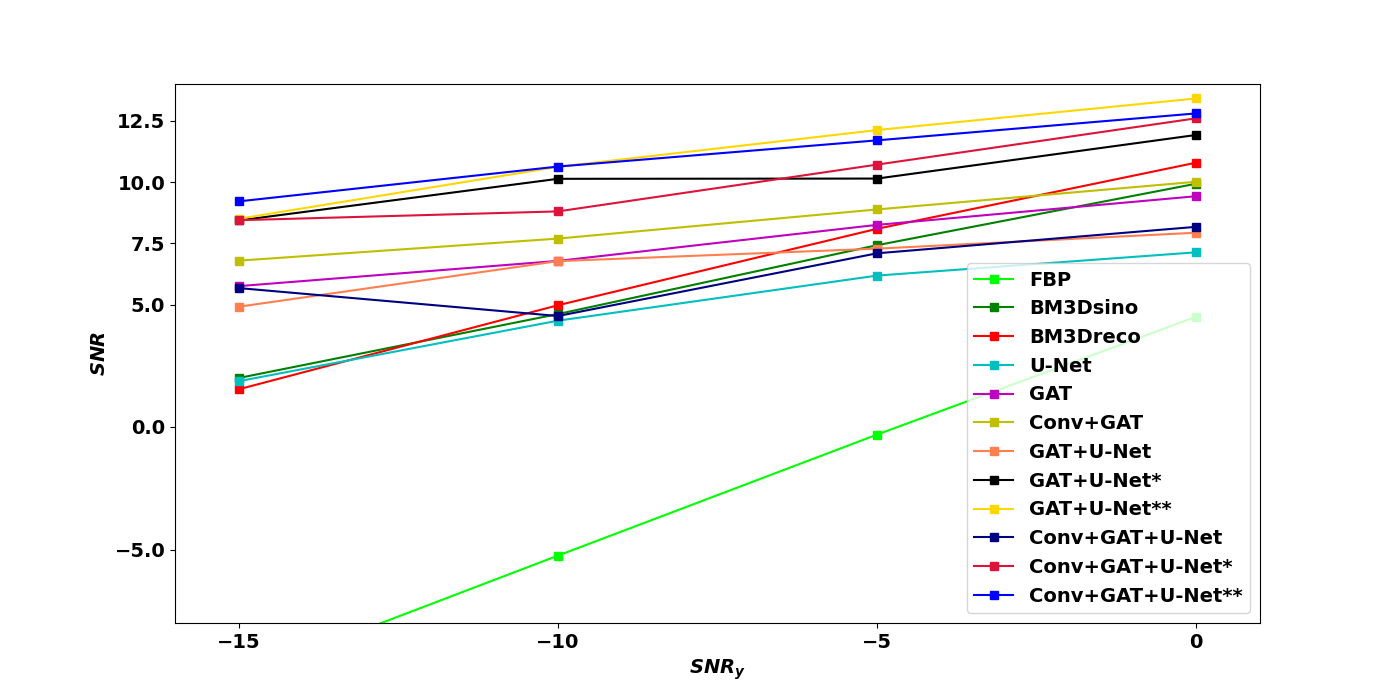
\includegraphics[width=0.8\textwidth]{small_components_result.png}
  \caption{
    Resulting SNR of different models and baseline algorithms.
    }
\end{figure}


\textbf{TODO: Add some visual results to Appendix.}


\section{Large Experiments}

\subsection{Baseline}
In Table~\ref{tab:baseline-large}, baseline results for large experiment can be found.
As algorithms are fixed, it is expected that the result is pretty close to the one from the small experiment.

\textbf{TODO: update with new numbers}

\begin{table}[H]
  \centering
  \begin{threeparttable}
    \begin{tabular}{l|cc|cc|cc|cc}
    \toprule
    \textbf{Algorithm} & \multicolumn{2}{l|}{\footnotesize \textbf{Input SNR 0 dB}} & \multicolumn{2}{l|}{\footnotesize \textbf{Input SNR -5 dB}} & \multicolumn{2}{l|}{\footnotesize \textbf{Input SNR -10 dB}} & \multicolumn{2}{l}{\footnotesize \textbf{Input SNR -15 dB}} \\
                       & \textbf{Loss} & \textbf{SNR} & \textbf{Loss} & \textbf{SNR} & \textbf{Loss} & \textbf{SNR} & \textbf{Loss} & \textbf{SNR} \\ 
    \midrule
    FBP                 &  1041.6          &  4.81            & 1772.8         & 0.0           & 3105.6          & -4.96          & 5495.2       & -9.94       \\ \hline
    BM3D sinogram       &  662.2           &  9.30            & 909.5          & 6.13          & 1285.2          & 2.93           & 1884.9       & -0.50       \\ \hline
    BM3D reconstruction &  \textbf{604.2}  &  \textbf{10.15}  & 840.4          & 6.81          & 1283.1          & 2.89           & 2079.1       & -1.42       \\ \hline
    U-Net               &  674.9           &  9.03            & \textbf{711.5} & \textbf{8.17} & \textbf{711.5}  & \textbf{8.17}  & \textbf{1224.9}       & \textbf{3.10}        \\ 
    \midrule
    \end{tabular}

  \end{threeparttable}

  \caption{Baseline results large experiments: Best result in column is marked bold. }
  \label{tab:baseline-large}
\end{table}

\textbf{TODO: Add some visual results to Appendix.}

\subsection{GAT-Denoiser components}

\textbf{TODO: Same same, but different. 20 epochs for all the models.}

\subsection{Last two models}

\textbf{TODO: Train for about 60 to 80 epochs and show best result.
Select best 2 models from above.}
